\documentclass{article}
\usepackage[T1]{fontenc}
\usepackage{lmodern}
\usepackage{graphicx}
\usepackage{amsmath,amssymb}
\usepackage[a4paper,margin=2cm]{geometry}
\usepackage[absolute,overlay]{textpos}
\setlength{\TPHorizModule}{1mm}
\setlength{\TPVertModule}{1mm}
\usepackage[indonesian]{babel}
\usepackage{hyperref}
\setlength{\emergencystretch}{2em}
% unit: Halaman 17

\begin{document}

% === Halaman 17 (llm) ===

\begin{itemize}
    \item Jika ordinat titik P nol, yaitu $y_p = \text{nol}$, maka tangen pada titik tersebut berpotongan pada sebuah titik di \textit{infinity}.
    \vspace{10mm}
    \item Di sini, $P + P = 2P = O$
\end{itemize}

\vspace{10mm}

\textcolor{red}{\text{Sumber gambar: Anoop MS, Elliptic Curve Cryptography, an Implementation Guide}}

% deskripsi: Grafik kurva eliptik yang menunjukkan titik P pada sumbu x dengan garis singgung vertikal yang menuju ke titik tak hingga (infinity), lengkap dengan keterangan teks y_p = 0 hence 2P = O.
% bbox normalisasi: [0.5130, 0.2740, 0.8010, 0.8940]
\begin{textblock*}{60.48mm}(107.73mm,81.38mm)
\noindent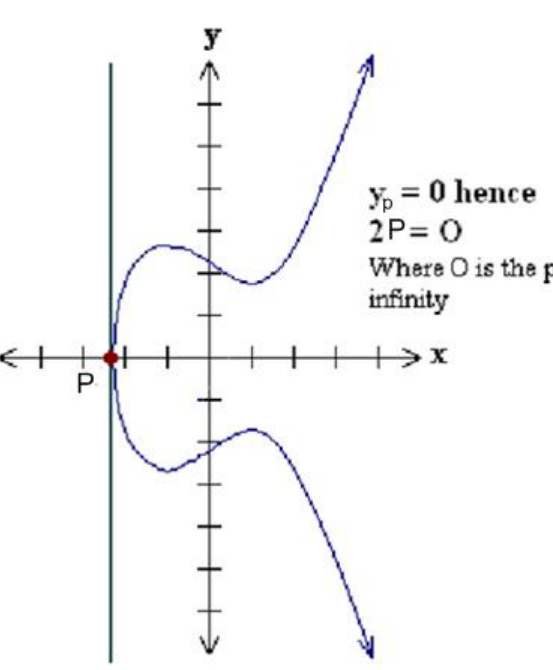
\includegraphics[width=60.48mm,height=184.14mm]{../../images/llm/page_017_img_01.png}%
\end{textblock*}

\end{document}
